% Generated by Sphinx.
\def\sphinxdocclass{report}
\documentclass[a4paper,10pt,english]{sphinxmanual}
\usepackage[utf8]{inputenc}
\DeclareUnicodeCharacter{00A0}{\nobreakspace}
\usepackage{cmap}
\usepackage[T1]{fontenc}
\usepackage{babel}
\usepackage{times}
\usepackage[Bjarne]{fncychap}
\usepackage{longtable}
\usepackage{sphinx}
\usepackage{multirow}

\usepackage{typo3}

\title{Datec Blog}
\date{2015-04-09 13:24}
\release{1.0.3}
\author{Philipp Roensch}
\newcommand{\sphinxlogo}{}
\renewcommand{\releasename}{Release}
\makeindex

\makeatletter
\def\PYG@reset{\let\PYG@it=\relax \let\PYG@bf=\relax%
    \let\PYG@ul=\relax \let\PYG@tc=\relax%
    \let\PYG@bc=\relax \let\PYG@ff=\relax}
\def\PYG@tok#1{\csname PYG@tok@#1\endcsname}
\def\PYG@toks#1+{\ifx\relax#1\empty\else%
    \PYG@tok{#1}\expandafter\PYG@toks\fi}
\def\PYG@do#1{\PYG@bc{\PYG@tc{\PYG@ul{%
    \PYG@it{\PYG@bf{\PYG@ff{#1}}}}}}}
\def\PYG#1#2{\PYG@reset\PYG@toks#1+\relax+\PYG@do{#2}}

\expandafter\def\csname PYG@tok@s1\endcsname{\def\PYG@tc##1{\textcolor[rgb]{0.25,0.44,0.63}{##1}}}
\expandafter\def\csname PYG@tok@nb\endcsname{\def\PYG@tc##1{\textcolor[rgb]{0.00,0.44,0.13}{##1}}}
\expandafter\def\csname PYG@tok@cm\endcsname{\let\PYG@it=\textit\def\PYG@tc##1{\textcolor[rgb]{0.25,0.50,0.56}{##1}}}
\expandafter\def\csname PYG@tok@ss\endcsname{\def\PYG@tc##1{\textcolor[rgb]{0.32,0.47,0.09}{##1}}}
\expandafter\def\csname PYG@tok@gd\endcsname{\def\PYG@tc##1{\textcolor[rgb]{0.63,0.00,0.00}{##1}}}
\expandafter\def\csname PYG@tok@mb\endcsname{\def\PYG@tc##1{\textcolor[rgb]{0.13,0.50,0.31}{##1}}}
\expandafter\def\csname PYG@tok@gp\endcsname{\let\PYG@bf=\textbf\def\PYG@tc##1{\textcolor[rgb]{0.78,0.36,0.04}{##1}}}
\expandafter\def\csname PYG@tok@ne\endcsname{\def\PYG@tc##1{\textcolor[rgb]{0.00,0.44,0.13}{##1}}}
\expandafter\def\csname PYG@tok@no\endcsname{\def\PYG@tc##1{\textcolor[rgb]{0.38,0.68,0.84}{##1}}}
\expandafter\def\csname PYG@tok@mh\endcsname{\def\PYG@tc##1{\textcolor[rgb]{0.13,0.50,0.31}{##1}}}
\expandafter\def\csname PYG@tok@err\endcsname{\def\PYG@bc##1{\setlength{\fboxsep}{0pt}\fcolorbox[rgb]{1.00,0.00,0.00}{1,1,1}{\strut ##1}}}
\expandafter\def\csname PYG@tok@vc\endcsname{\def\PYG@tc##1{\textcolor[rgb]{0.73,0.38,0.84}{##1}}}
\expandafter\def\csname PYG@tok@gh\endcsname{\let\PYG@bf=\textbf\def\PYG@tc##1{\textcolor[rgb]{0.00,0.00,0.50}{##1}}}
\expandafter\def\csname PYG@tok@o\endcsname{\def\PYG@tc##1{\textcolor[rgb]{0.40,0.40,0.40}{##1}}}
\expandafter\def\csname PYG@tok@kc\endcsname{\let\PYG@bf=\textbf\def\PYG@tc##1{\textcolor[rgb]{0.00,0.44,0.13}{##1}}}
\expandafter\def\csname PYG@tok@sb\endcsname{\def\PYG@tc##1{\textcolor[rgb]{0.25,0.44,0.63}{##1}}}
\expandafter\def\csname PYG@tok@gi\endcsname{\def\PYG@tc##1{\textcolor[rgb]{0.00,0.63,0.00}{##1}}}
\expandafter\def\csname PYG@tok@kd\endcsname{\let\PYG@bf=\textbf\def\PYG@tc##1{\textcolor[rgb]{0.00,0.44,0.13}{##1}}}
\expandafter\def\csname PYG@tok@s\endcsname{\def\PYG@tc##1{\textcolor[rgb]{0.25,0.44,0.63}{##1}}}
\expandafter\def\csname PYG@tok@nf\endcsname{\def\PYG@tc##1{\textcolor[rgb]{0.02,0.16,0.49}{##1}}}
\expandafter\def\csname PYG@tok@k\endcsname{\let\PYG@bf=\textbf\def\PYG@tc##1{\textcolor[rgb]{0.00,0.44,0.13}{##1}}}
\expandafter\def\csname PYG@tok@w\endcsname{\def\PYG@tc##1{\textcolor[rgb]{0.73,0.73,0.73}{##1}}}
\expandafter\def\csname PYG@tok@c\endcsname{\let\PYG@it=\textit\def\PYG@tc##1{\textcolor[rgb]{0.25,0.50,0.56}{##1}}}
\expandafter\def\csname PYG@tok@sr\endcsname{\def\PYG@tc##1{\textcolor[rgb]{0.14,0.33,0.53}{##1}}}
\expandafter\def\csname PYG@tok@ge\endcsname{\let\PYG@it=\textit}
\expandafter\def\csname PYG@tok@gr\endcsname{\def\PYG@tc##1{\textcolor[rgb]{1.00,0.00,0.00}{##1}}}
\expandafter\def\csname PYG@tok@nt\endcsname{\let\PYG@bf=\textbf\def\PYG@tc##1{\textcolor[rgb]{0.02,0.16,0.45}{##1}}}
\expandafter\def\csname PYG@tok@c1\endcsname{\let\PYG@it=\textit\def\PYG@tc##1{\textcolor[rgb]{0.25,0.50,0.56}{##1}}}
\expandafter\def\csname PYG@tok@nc\endcsname{\let\PYG@bf=\textbf\def\PYG@tc##1{\textcolor[rgb]{0.05,0.52,0.71}{##1}}}
\expandafter\def\csname PYG@tok@mo\endcsname{\def\PYG@tc##1{\textcolor[rgb]{0.13,0.50,0.31}{##1}}}
\expandafter\def\csname PYG@tok@sx\endcsname{\def\PYG@tc##1{\textcolor[rgb]{0.78,0.36,0.04}{##1}}}
\expandafter\def\csname PYG@tok@il\endcsname{\def\PYG@tc##1{\textcolor[rgb]{0.13,0.50,0.31}{##1}}}
\expandafter\def\csname PYG@tok@m\endcsname{\def\PYG@tc##1{\textcolor[rgb]{0.13,0.50,0.31}{##1}}}
\expandafter\def\csname PYG@tok@ow\endcsname{\let\PYG@bf=\textbf\def\PYG@tc##1{\textcolor[rgb]{0.00,0.44,0.13}{##1}}}
\expandafter\def\csname PYG@tok@vg\endcsname{\def\PYG@tc##1{\textcolor[rgb]{0.73,0.38,0.84}{##1}}}
\expandafter\def\csname PYG@tok@vi\endcsname{\def\PYG@tc##1{\textcolor[rgb]{0.73,0.38,0.84}{##1}}}
\expandafter\def\csname PYG@tok@se\endcsname{\let\PYG@bf=\textbf\def\PYG@tc##1{\textcolor[rgb]{0.25,0.44,0.63}{##1}}}
\expandafter\def\csname PYG@tok@gt\endcsname{\def\PYG@tc##1{\textcolor[rgb]{0.00,0.27,0.87}{##1}}}
\expandafter\def\csname PYG@tok@go\endcsname{\def\PYG@tc##1{\textcolor[rgb]{0.20,0.20,0.20}{##1}}}
\expandafter\def\csname PYG@tok@kn\endcsname{\let\PYG@bf=\textbf\def\PYG@tc##1{\textcolor[rgb]{0.00,0.44,0.13}{##1}}}
\expandafter\def\csname PYG@tok@mi\endcsname{\def\PYG@tc##1{\textcolor[rgb]{0.13,0.50,0.31}{##1}}}
\expandafter\def\csname PYG@tok@bp\endcsname{\def\PYG@tc##1{\textcolor[rgb]{0.00,0.44,0.13}{##1}}}
\expandafter\def\csname PYG@tok@ni\endcsname{\let\PYG@bf=\textbf\def\PYG@tc##1{\textcolor[rgb]{0.84,0.33,0.22}{##1}}}
\expandafter\def\csname PYG@tok@s2\endcsname{\def\PYG@tc##1{\textcolor[rgb]{0.25,0.44,0.63}{##1}}}
\expandafter\def\csname PYG@tok@si\endcsname{\let\PYG@it=\textit\def\PYG@tc##1{\textcolor[rgb]{0.44,0.63,0.82}{##1}}}
\expandafter\def\csname PYG@tok@sh\endcsname{\def\PYG@tc##1{\textcolor[rgb]{0.25,0.44,0.63}{##1}}}
\expandafter\def\csname PYG@tok@gs\endcsname{\let\PYG@bf=\textbf}
\expandafter\def\csname PYG@tok@kt\endcsname{\def\PYG@tc##1{\textcolor[rgb]{0.56,0.13,0.00}{##1}}}
\expandafter\def\csname PYG@tok@nl\endcsname{\let\PYG@bf=\textbf\def\PYG@tc##1{\textcolor[rgb]{0.00,0.13,0.44}{##1}}}
\expandafter\def\csname PYG@tok@kp\endcsname{\def\PYG@tc##1{\textcolor[rgb]{0.00,0.44,0.13}{##1}}}
\expandafter\def\csname PYG@tok@gu\endcsname{\let\PYG@bf=\textbf\def\PYG@tc##1{\textcolor[rgb]{0.50,0.00,0.50}{##1}}}
\expandafter\def\csname PYG@tok@nn\endcsname{\let\PYG@bf=\textbf\def\PYG@tc##1{\textcolor[rgb]{0.05,0.52,0.71}{##1}}}
\expandafter\def\csname PYG@tok@nd\endcsname{\let\PYG@bf=\textbf\def\PYG@tc##1{\textcolor[rgb]{0.33,0.33,0.33}{##1}}}
\expandafter\def\csname PYG@tok@sc\endcsname{\def\PYG@tc##1{\textcolor[rgb]{0.25,0.44,0.63}{##1}}}
\expandafter\def\csname PYG@tok@na\endcsname{\def\PYG@tc##1{\textcolor[rgb]{0.25,0.44,0.63}{##1}}}
\expandafter\def\csname PYG@tok@cs\endcsname{\def\PYG@tc##1{\textcolor[rgb]{0.25,0.50,0.56}{##1}}\def\PYG@bc##1{\setlength{\fboxsep}{0pt}\colorbox[rgb]{1.00,0.94,0.94}{\strut ##1}}}
\expandafter\def\csname PYG@tok@kr\endcsname{\let\PYG@bf=\textbf\def\PYG@tc##1{\textcolor[rgb]{0.00,0.44,0.13}{##1}}}
\expandafter\def\csname PYG@tok@cp\endcsname{\def\PYG@tc##1{\textcolor[rgb]{0.00,0.44,0.13}{##1}}}
\expandafter\def\csname PYG@tok@mf\endcsname{\def\PYG@tc##1{\textcolor[rgb]{0.13,0.50,0.31}{##1}}}
\expandafter\def\csname PYG@tok@nv\endcsname{\def\PYG@tc##1{\textcolor[rgb]{0.73,0.38,0.84}{##1}}}
\expandafter\def\csname PYG@tok@sd\endcsname{\let\PYG@it=\textit\def\PYG@tc##1{\textcolor[rgb]{0.25,0.44,0.63}{##1}}}

\def\PYGZbs{\char`\\}
\def\PYGZus{\char`\_}
\def\PYGZob{\char`\{}
\def\PYGZcb{\char`\}}
\def\PYGZca{\char`\^}
\def\PYGZam{\char`\&}
\def\PYGZlt{\char`\<}
\def\PYGZgt{\char`\>}
\def\PYGZsh{\char`\#}
\def\PYGZpc{\char`\%}
\def\PYGZdl{\char`\$}
\def\PYGZhy{\char`\-}
\def\PYGZsq{\char`\'}
\def\PYGZdq{\char`\"}
\def\PYGZti{\char`\~}
% for compatibility with earlier versions
\def\PYGZat{@}
\def\PYGZlb{[}
\def\PYGZrb{]}
\makeatother

\renewcommand\PYGZsq{\textquotesingle}

\begin{document}

\maketitle
\tableofcontents
\phantomsection\label{Index::doc}



\chapter{What does it do?}
\label{Introduction/Index:introduction}\label{Introduction/Index:what-does-it-do}\label{Introduction/Index:start}\label{Introduction/Index:datec-blog}\label{Introduction/Index::doc}
This extension gives you a lightweight, yet modern Blog to add to your homepage.
The Extension will add a frontend plugin with various display types that allow the following features:
\begin{itemize}
\item {} 
Blog system with posts, categories and keywords

\item {} 
Write text and add images to your blogpost

\item {} 
Write a teaser text and/or choose a teaser image for the blogpost

\item {} 
Organize blogposts in categories and assign multiple keywords

\item {} 
Displays categries as tree

\item {} 
As well as the generated archive

\item {} 
Keywords are displayed as cloud or list, highlighted by click count

\item {} 
Bloglist can be filtered by categories, archive period or keywords

\item {} 
Blogposts in singleview display comments hierarchically

\item {} 
User access to comments can be disabled entirely or controlled with frontend user groups for each blogpost

\item {} 
Comments may contain file uploads

\item {} 
Commenting is spam protected internally for barrier-free usage

\item {} 
Commenting users are saved with username and email-address or frontend user id and can be blocked individually

\item {} 
Default HTML markup matches Twitter Bootstrap 3

\end{itemize}

\begin{notice}{tip}{Tip:}
Visit \& contribute: \href{https://github.com/theorak/DatecBlog}{https://github.com/theorak/DatecBlog}
\end{notice}
\begin{figure}[htbp]
\centering
\capstart

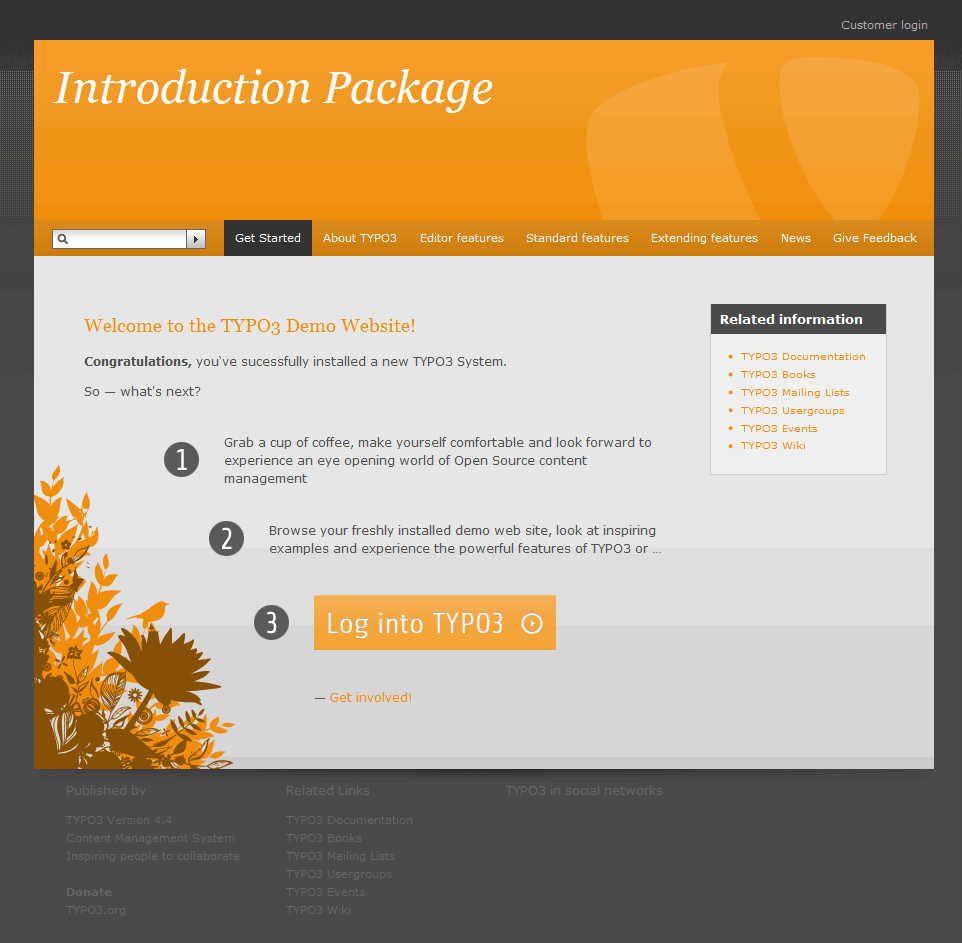
\includegraphics{IntroductionPackage.png}
\caption{Introduction Package just after installation (caption of the image)}{\small 
How the Frontend of the Introduction Package looks like just after installation (legend of the image)
}\end{figure}


\chapter{Users manual}
\label{UsersManual/Index:users-manual}\label{UsersManual/Index::doc}\label{UsersManual/Index:id1}
Target group: \textbf{Editors and Users}


\section{Editors - Create a category}
\label{UsersManual/Index:editors-create-a-category}\begin{itemize}
\item {} 
Name: name of the category, musn't be numbered

\item {} 
Parent Category: (optional) choose the parent category to build a hierachy

\item {} 
Disabled: hide/display this category

\item {} 
Usergroups: control user access to this category AND all blogposts assigned to it

\end{itemize}
\begin{figure}[htbp]
\centering
\capstart

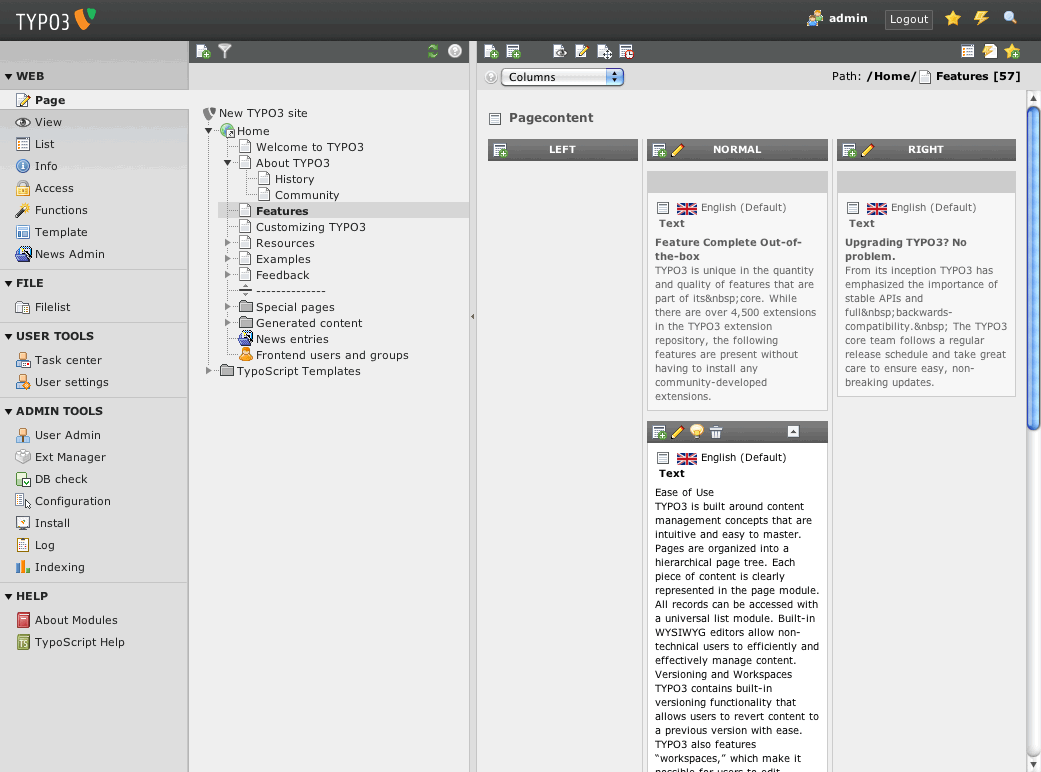
\includegraphics{BackendView.png}
\caption{Default Backend view (caption of the image)}{\small 
The Backend view of TYPO3 after the user has clicked on module ``Page''. (legend of the image)
}\end{figure}


\section{Editors - Create a blogpost}
\label{UsersManual/Index:editors-create-a-blogpost}\begin{itemize}
\item {} 
Title: title of the blogpost

\item {} 
Blog-Text: write the main blog content

\item {} 
Category: set a category that fits this blogpost

\item {} 
Keywords: add one or more keywords associated with the blogpost (see next step for details on keywords)

\item {} 
Images: add references to images (like on content elements), these will be displayed with a preview to click-enlarge below the post

\item {} 
Disabled: hide/display this blogpost

\item {} 
Start/Stop: controll visibility further with access times

\item {} 
Disable Comments: will ignore settings below and just disable comments altogether

\item {} 
Allow File Uploads on Comments: adds a file upload field to the comment form

\item {} 
Comments Usergroups: control user access to COMMENT on this blogpost (NOT VISIBILITY)

\end{itemize}
\begin{figure}[htbp]
\centering
\capstart

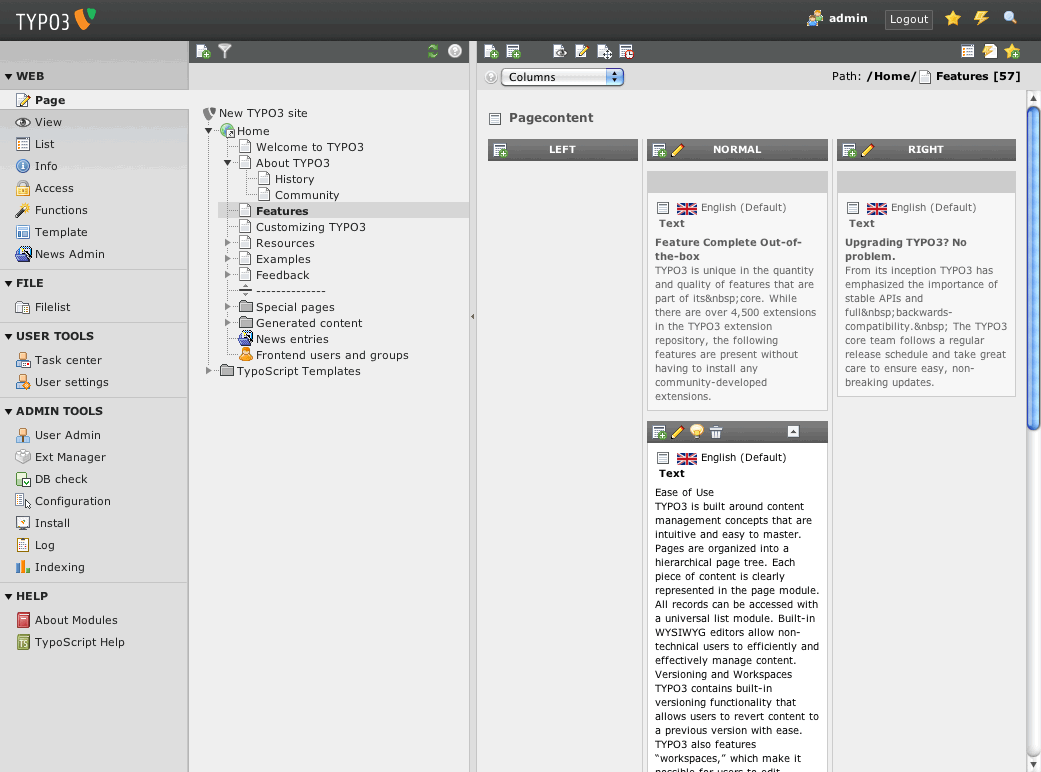
\includegraphics{BackendView.png}
\caption{Default Backend view (caption of the image)}{\small 
The Backend view of TYPO3 after the user has clicked on module ``Page''. (legend of the image)
}\end{figure}


\section{Editors - Create a keyword}
\label{UsersManual/Index:editors-create-a-keyword}\begin{itemize}
\item {} 
Disabled: hide/display this keyword

\item {} 
Word: the keyword

\item {} 
Posts: (optional) choose blogposts to assign this keyword to (might also be done on the blogposts themselves)

\item {} 
Usage (click count): see and manipulate the usage of a keyword to highlight it

\end{itemize}
\begin{figure}[htbp]
\centering
\capstart

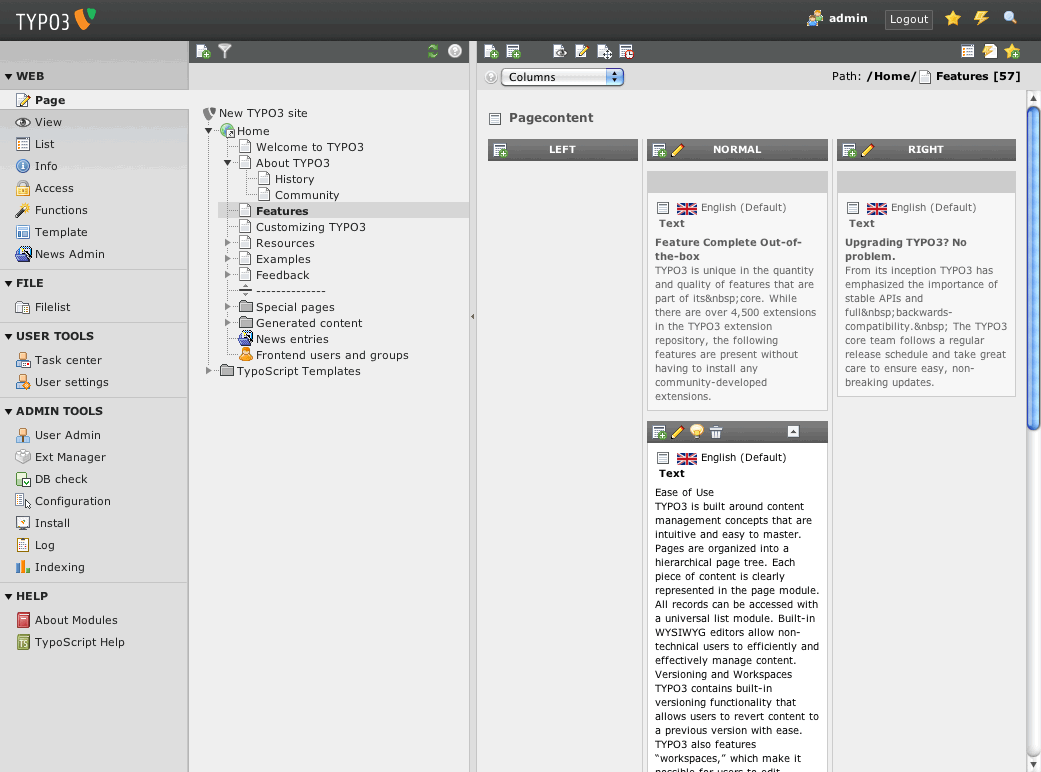
\includegraphics{BackendView.png}
\caption{Default Backend view (caption of the image)}{\small 
The Backend view of TYPO3 after the user has clicked on module ``Page''. (legend of the image)
}\end{figure}


\section{Editors - Edit/Inspect a comment creator}
\label{UsersManual/Index:editors-edit-inspect-a-comment-creator}
Comment creators are generated by the plugin to relate between frontend users and comments or to save a public user. The editors may want to inspect these creators to access their email-address, or block them to prevent them from commenting. Comment creators should never have to be deleted.
\begin{itemize}
\item {} 
Disabled: hide/display this comment creator

\item {} 
Homepage User: contains a reference to the frontent user if he created a comment

\item {} 
Username: username as entered by the user

\item {} 
Email-Address: email-address as entered by the user, is validated

\item {} 
Block from commenting: does exactly that

\end{itemize}
\begin{figure}[htbp]
\centering
\capstart

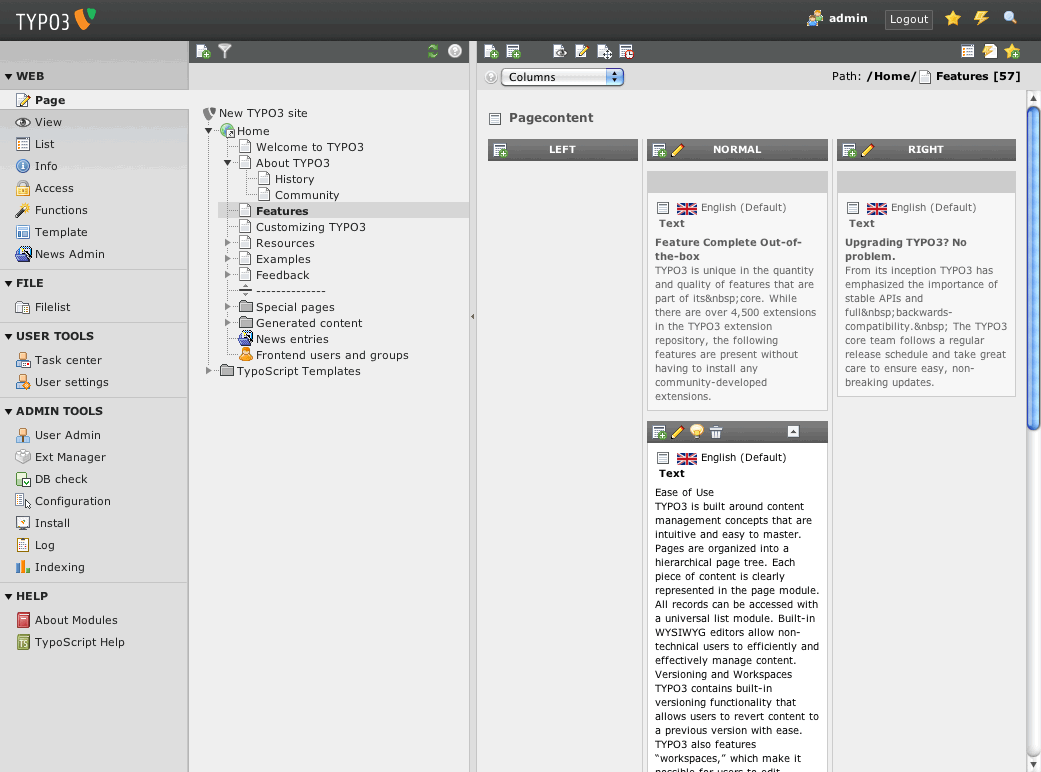
\includegraphics{BackendView.png}
\caption{Default Backend view (caption of the image)}{\small 
The Backend view of TYPO3 after the user has clicked on module ``Page''. (legend of the image)
}\end{figure}


\section{Users - Bloglist and Filter}
\label{UsersManual/Index:users-bloglist-and-filter}
The bloglist is the initial view, it shows the titles, teasertext (optional), teaserimage (optional) and the latest comment (if any), plus the category and keywords assigned with this blogpost.
This list can be filtered by clicking the categories, an archive period or keywords, easily selectable with the tree views on the same page. Clicking on anything with a hand cursor will add or remove it to the filter, or the `Clear Filter' button will empty the filter completly.
\begin{figure}[htbp]
\centering
\capstart

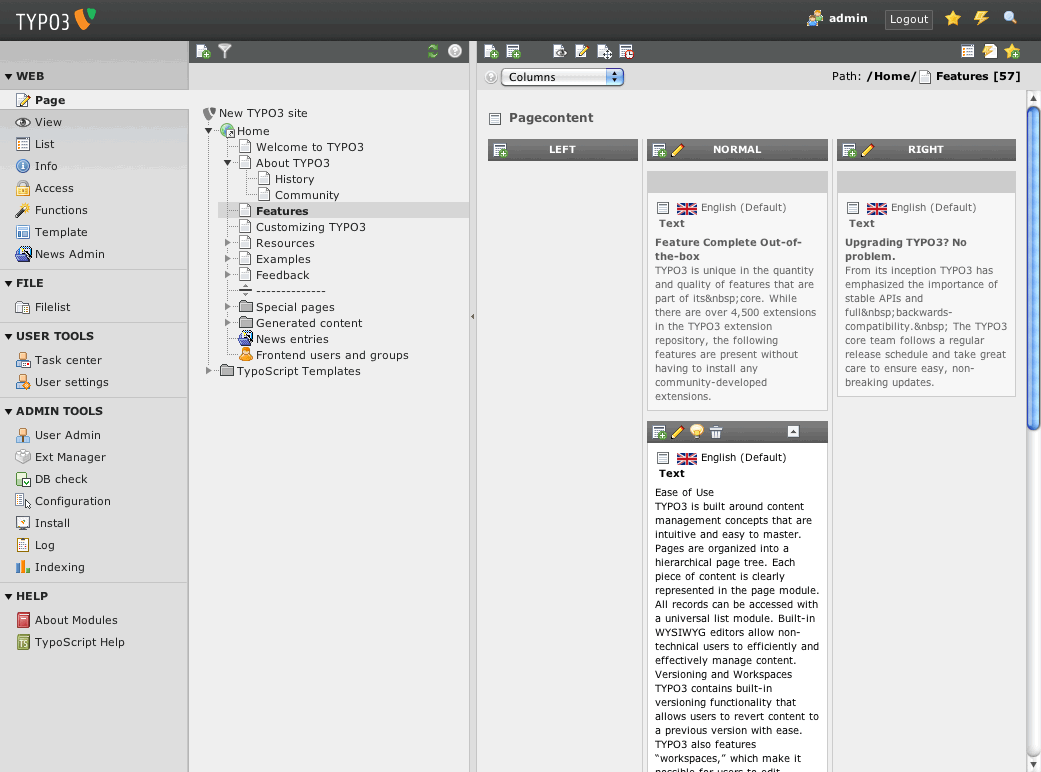
\includegraphics{BackendView.png}
\caption{Default Backend view (caption of the image)}{\small 
The Backend view of TYPO3 after the user has clicked on module ``Page''. (legend of the image)
}\end{figure}


\section{Users - Blogpost and Comments}
\label{UsersManual/Index:users-blogpost-and-comments}
To open a blogpost in single view, simply click it's title. The single view will show the full blogpost text and images and a hierarchial list of comments below.

Users can comment by using the form, public users enter their username and email-address, logged-in users have this form prefilled. Logged-in backend users can ignore that and will just appear as the user creating this comment. The `reply' button after each comment will add this comment as a reference to the form (see text in screenshot) and can be removed by clicking the reference. This form is spam protected with an internal check.


\section{Users/Editors - Advanced Blog Usage}
\label{UsersManual/Index:users-editors-advanced-blog-usage}
Linking directly into the blog can be done with the following easy parameters, just add them to your URL (pointing at the Blog Page):

\begin{tabulary}{\linewidth}{|L|L|}
\hline
\textsf{\relax 
Parameter
} & \textsf{\relax 
Links to
}\\
\hline
\&blogpost=\textless{}ID\textgreater{}
 & 
directly to blogpost, via ID
\\
\hline
\#tx-datec-blog-comment-\textless{}ID\textgreater{}
 & 
focus on comment, with ID
\\
\hline
\#tx-datec-blog-comments
 & 
focus on comment section
\\
\hline\end{tabulary}



\chapter{Administrator Manual}
\label{AdministratorManual/Index:administrator-manual}\label{AdministratorManual/Index::doc}\label{AdministratorManual/Index:admin-manual}
Target group: \textbf{Administrators}


\section{Requirements}
\label{AdministratorManual/Index:requirements}
\begin{notice}{caution}{Caution:}
You must load the jQuery JavaScript framework yourself as the frontend plugin utilizes functions that depend on jQuery.
\end{notice}


\section{Installation}
\label{AdministratorManual/Index:installation}\begin{enumerate}
\item {} 
Download and install the extension via the extension manager (extKey: datec\_blog).

\item {} 
Add one storage folder for comments and comment creators, note down the page id (PID) of this folder.

\item {} 
Check the Configuration section of this manual for the required configuration and follow the steps there.

\item {} 
Insert the main plugin and optional ones as described below.

\end{enumerate}


\section{Insert plugin}
\label{AdministratorManual/Index:insert-plugin}\begin{enumerate}
\item {} 
Insert a content element, choose ``Plugins'' -\textgreater{} ``General Plugin''

\end{enumerate}
\begin{figure}[htbp]
\centering

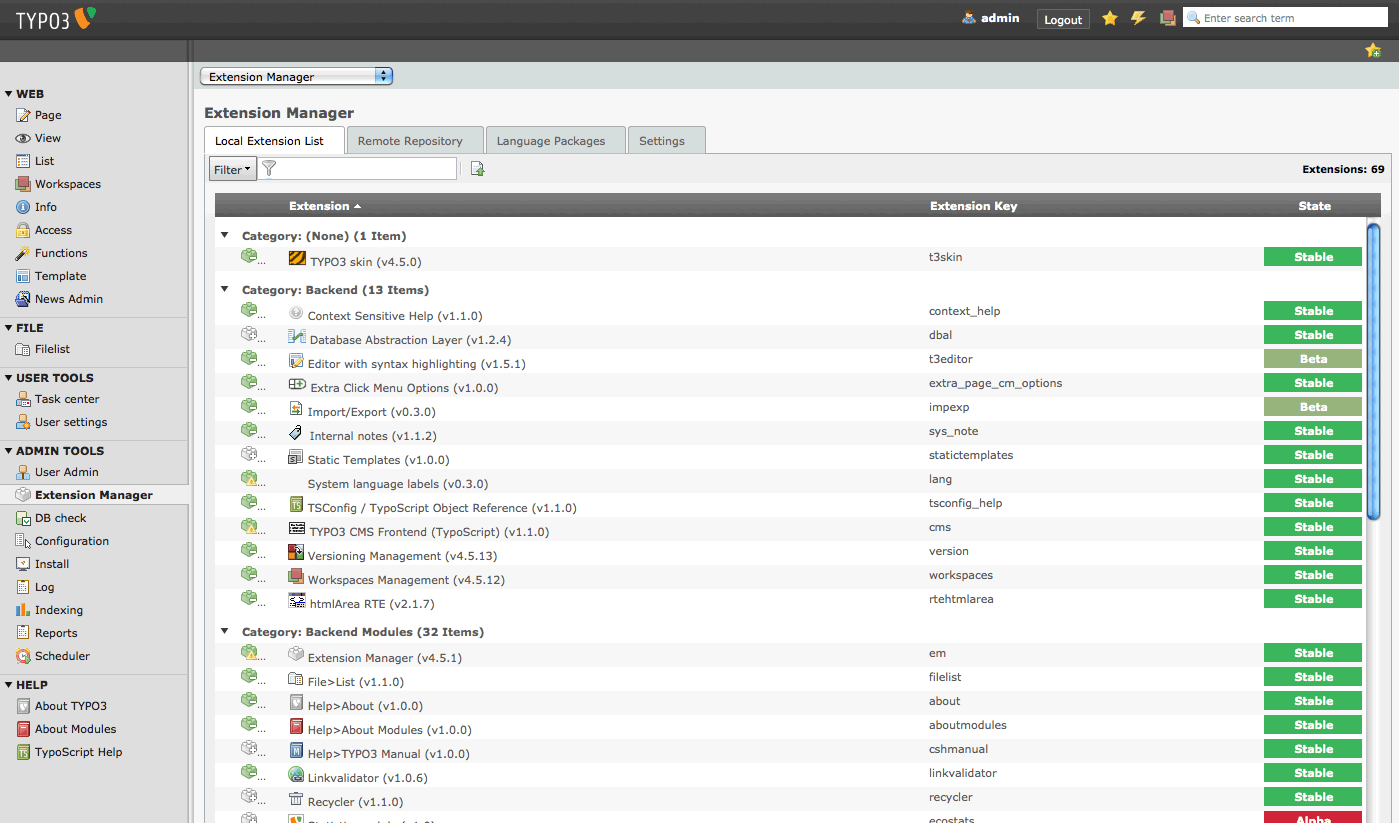
\includegraphics{ExtensionManager.png}
\end{figure}
\begin{enumerate}
\setcounter{enumi}{1}
\item {} 
Choose one of the display forms to setup your blog.

\end{enumerate}
\begin{figure}[htbp]
\centering
\capstart

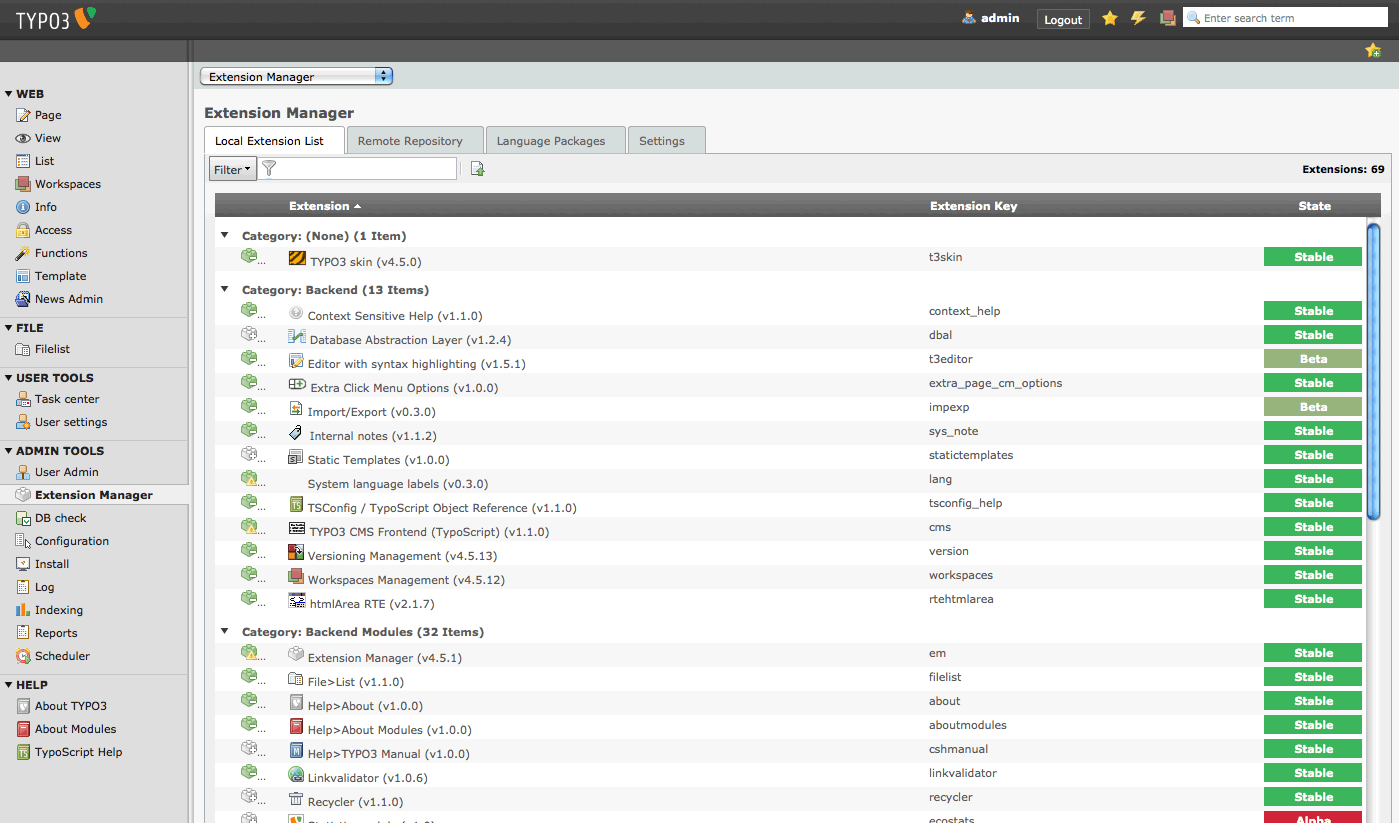
\includegraphics{ExtensionManager.png}
\caption{Modules}\end{figure}


\subsection{Blog}
\label{AdministratorManual/Index:blog}
Displays a the bloglist with filter and single view of posts with comments. This Plugin is required.


\subsection{Categories}
\label{AdministratorManual/Index:categories}
Displays Categories as a tree, clickable for the filter.


\subsection{Archive}
\label{AdministratorManual/Index:archive}
Generates an Archive from all Blogposts, displayed as tree of year - month - day, clickable for the filter.


\subsection{Keywords}
\label{AdministratorManual/Index:keywords}
Displays Keywords as cloud or list, depending on your plugin TypoScript configuration, clickable for the filter.

Target group: \textbf{Administrators}


\chapter{Configuration Reference}
\label{Configuration/Index:configuration}\label{Configuration/Index:configuration-reference}\label{Configuration/Index::doc}
This section describes all options aviable for Datec Blog via TypoScript setup. To change these options please add a new extension template to your ROOT template.


\section{Minimal configuration}
\label{Configuration/Index:configuration-typoscript}\label{Configuration/Index:minimal-configuration}
Upon installation, please add the static extension template `Datec Blog' to your ROOT template (Web \textgreater{} Template \textgreater{} edit root page template \textgreater{} Includes \textgreater{} select static template from extensions) and set at least the following options:

\begin{Verbatim}[frame=single,commandchars=\\\{\}]
\PYGZsh{} PID of your storage folder for comments and comment creators
plugin.tx\PYGZus{}datecblog\PYGZus{}blog.settings.commentsStoragePid = 123

\PYGZsh{} Valid email address to dispatch automatic mails from
plugin.tx\PYGZus{}datecblog\PYGZus{}blog.settings.mail.internMailFrom = blog@no\PYGZhy{}reply.com
\end{Verbatim}


\section{General configuration}
\label{Configuration/Index:general-configuration}
plugin.tx\_datecblog\_blog.

\begin{longtable}{|l|l|l|l|}
\hline
\textsf{\relax 
Property
} & \textsf{\relax 
Data type
} & \textsf{\relax 
Description
} & \textsf{\relax 
Default
}\\
\hline\endfirsthead

\multicolumn{4}{c}%
{{\textsf{\tablename\ \thetable{} -- continued from previous page}}} \\
\hline
\textsf{\relax 
Property
} & \textsf{\relax 
Data type
} & \textsf{\relax 
Description
} & \textsf{\relax 
Default
}\\
\hline\endhead

\hline \multicolumn{4}{|r|}{{\textsf{Continued on next page}}} \\ \hline
\endfoot

\endlastfoot


view.templateRootPath
 & 
string
 & 
Constant, path to template files if you wish to use your own.
 & 
EXT:datec\_blog/Resources/Private/Templates/
\\
\hline
view.partialRootPath
 & 
string
 & 
Constant, path to partial template files if you wish to use your own.
 & 
EXT:datec\_blog/Resources/Private/Partials/
\\
\hline
view.layoutRootPath
 & 
string
 & 
Constant, path to layout files if you wish to use your own.
 & 
EXT:datec\_blog/Resources/Private/Layouts/
\\
\hline
settings.commentsStoragePid
 & 
int
 & 
System folder for comments and comment creators.
 & \\
\hline
settings.mail.internMailFrom
 & 
string
 & 
E-mail address for automatic notification Mails {[}FROM{]}.
 & 
\href{mailto:blog@no-reply.com}{blog@no-reply.com}
\\
\hline
settings.mail.internMailFromName
 & 
string
 & 
Name to display for automatic notification Mails {[}FROM-NAME{]}.
 & 
Datec Blog
\\
\hline
settings.maxFileSize
 & 
string
 & 
Maximum file size in bytes on comments with file attachments.
 & 
4000000
\\
\hline
settings.allowedFileTypes
 & 
string
 & 
File types allowed, listing comma-separated, on comments with file upload.
 & 
pdf,zip,png,jpg,jpeg,gif,txt,doc,docx
\\
\hline
settings.display.dateFormat
 & 
string
 & 
Date format to display dates, must be compatible to date() PHP function.
 & 
d.m.Y
\\
\hline
settings.display.showDefaultHeaders
 & 
boolean
 & 
Display Titles about each plugin (e.g. `Categories').
 & 
1
\\
\hline
settings.display.keywords.limit
 & 
string
 & 
Limit keyword results to this number, set 0 to disable.
 & 
0
\\
\hline
settings.display.keywords.order
 & 
string
 & 
Order keywords by `date', `usage' or `sorting'.
 & 
usage
\\
\hline
settings.display.keywords.visual
 & 
string
 & 
Display keywords as `cloud' or `list'.
 & 
cloud
\\
\hline
settings.display.posts.dateFormat
 & 
string
 & 
Like `settings.display.dateFormat' for posts only.
 & 
d.m.Y - H:i
\\
\hline
settings.display.posts.teaserTextLength
 & 
string
 & 
Blogposts (without teasertext) will be cut of at this length in list view.
 & 
40
\\
\hline
settings.display.posts.sorting
 & 
string
 & 
Column name for SQL-query to sort blogposts by.
 & 
crdate
\\
\hline
settings.display.posts.sortingDirection
 & 
string
 & 
Sorting direction for SQL-query to sort blogposts by.
 & 
DESC
\\
\hline
settings.display.posts.pagination.enable
 & 
boolean
 & 
Enable pagination for bloglist.
 & 
1
\\
\hline
settings.display.posts.pagination.itemsPerPage
 & 
int
 & 
Blogposts per page.
 & 
15
\\
\hline
settings.display.posts.pagination.maxPages
 & 
int
 & 
Maximum Pages displayed, 0 disables this. (reduces visible content!)
 & 
0
\\
\hline
settings.display.posts.pagination.top
 & 
boolean
 & 
Pagination should appear above the bloglist.
 & 
0
\\
\hline
settings.display.posts.pagination.bottom
 & 
boolean
 & 
Pagination should appear below the bloglist.
 & 
1
\\
\hline
settings.display.comments.dateFormat
 & 
string
 & 
Like `settings.display.dateFormat' for comments only.
 & 
d.m.Y - H:i
\\
\hline
settings.display.comments.sorting
 & 
string
 & 
Sorting direction for SQL-query to sort comments by.
 & 
crdate
\\
\hline
settings.display.comments.sortingDirection
 & 
string
 & 
Sorting direction for SQL-query to sort comments by.
 & 
DESC
\\
\hline
settings.display.feUser.nameFormat
 & 
string
 & 
Display user with `username', `firstname\_lastname', `firstname' or `lastname'.
 & 
username
\\
\hline
settings.cssClasses.form
 & 
string
 & 
CSS class for forms. (All CSS-settings are suggested Bootstrap default)
 & 
form form-inline
\\
\hline
settings.cssClasses.formLabel
 & 
string
 & 
CSS class for form labels.
 & 
control-label
\\
\hline
settings.cssClasses.formField
 & 
string
 & 
CSS class for form fields.
 & 
form-control
\\
\hline
settings.cssClasses.formFieldWrap
 & 
string
 & 
CSS class to wrap around fields + label.
 & 
form-group
\\
\hline
settings.cssClasses.formButton
 & 
string
 & 
CSS class for form buttons.
 & 
btn btn-default
\\
\hline
settings.cssClasses.listGroup
 & 
string
 & 
CSS class for list groups (`ul').
 & \\
\hline
settings.cssClasses.listItem
 & 
string
 & 
CSS class for list items(`li').
 & \\
\hline\end{longtable}



\chapter{Known Problems}
\label{KnownProblems/Index:known-problems}\label{KnownProblems/Index::doc}\label{KnownProblems/Index:id1}
No problems reported yet.

Issues will be tracked \href{https://github.com/theorak/DatecBlog}{here}


\chapter{To-Do List}
\label{ToDoList/Index:to-do-list}\label{ToDoList/Index::doc}\label{ToDoList/Index:id1}
All is well.

See current development \href{https://github.com/theorak/DatecBlog}{here}


\chapter{Change Log}
\label{ChangeLog/Index:change-log}\label{ChangeLog/Index::doc}\label{ChangeLog/Index:id1}
Changes will be tracked \href{https://github.com/theorak/DatecBlog}{here}.


\chapter{FAQ}
\label{FAQ/Index::doc}\label{FAQ/Index:faq}\label{FAQ/Index:id1}

\section{How to change the layout/design?}
\label{FAQ/Index:how-to-change-the-layout-design}
Copy the template files (\code{datec\_blog\textbackslash{}Resources\textbackslash{}Private\textbackslash{}Layouts} \textbackslash{}Partials, \textbackslash{}Templates)
into the fileadmin folder and change the paths via TS or constant editor (see the configuration section of this document).



\renewcommand{\indexname}{Index}
\printindex
\end{document}
